\documentclass[10pt,a4paper]{article}
\usepackage[a4paper,top=18mm,bottom=18mm,left=18mm,right=18mm]{geometry}
\usepackage[T1]{fontenc}
\usepackage{newtxtext,newtxmath}
\usepackage{microtype}
\usepackage{booktabs}
\usepackage{longtable}
\usepackage{array}
\usepackage{tabularx}
\usepackage{graphicx}
\usepackage[hidelinks]{hyperref}
\usepackage{xurl}
\usepackage{xcolor}
\usepackage{caption}
\usepackage{fancyhdr}
\usepackage{needspace}
\hypersetup{
  pdftitle={Supplementary Information for ReRAPTOR},
  pdfauthor={Bin Zhou, Guangxian Li, Teruki Ogo, Yutaka Arakawa, and Tsunenori Mine}
}

\setlength{\parindent}{0pt}
\setlength{\parskip}{3pt}
\setlength{\tabcolsep}{3.5pt}
\renewcommand{\arraystretch}{1.10}
\raggedbottom
\pagestyle{fancy}
\fancyhf{}
\fancyhead[L]{\footnotesize ReRAPTOR}
\fancyhead[R]{\footnotesize Supplementary Information}
\fancyfoot[C]{\footnotesize S\thepage}
\renewcommand{\headrulewidth}{0.4pt}
\renewcommand{\footrulewidth}{0pt}
\setlength{\headheight}{13pt}
\newcommand{\ci}[2]{[#1, #2]}
\newcommand{\suppheading}[2]{%
  \par\needspace{7\baselineskip}\vspace{8pt}%
  {\large\bfseries Supplementary #1. #2}\par\vspace{5pt}}
\newcommand{\panel}[1]{\par\vspace{5pt}\textit{#1}\par\smallskip}
\newcommand{\sourcefile}[1]{%
  \par\vspace{1pt}{\footnotesize\raggedright\textit{Source:} \texttt{#1}\par}}

\begin{document}

\begin{center}
{\small\bfseries SUPPLEMENTARY INFORMATION}\par\vspace{6pt}
{\LARGE\bfseries ReRAPTOR: Reverse-Objective RAPTOR for Time-Budgeted\par
Value-Maximizing Transit Itinerary Planning}\par\vspace{8pt}
{\large Bin Zhou\textsuperscript{1}, Guangxian Li\textsuperscript{1},
Teruki Ogo\textsuperscript{2}, Yutaka Arakawa\textsuperscript{1}, and
Tsunenori Mine\textsuperscript{1}}\par\vspace{5pt}
{\small
\textsuperscript{1}Graduate School of Information Science and Electrical Engineering,
Kyushu University, Fukuoka, Japan\\
\textsuperscript{2}Faculty of Information Science and Engineering,
Kyushu Sangyo University, Fukuoka, Japan}
\end{center}
\vspace{4pt}\hrule\vspace{8pt}

These tables provide a visible numerical source for detailed values cited in
the manuscript. Unless noted otherwise, a gap is ReRAPTOR minus NSGA-II, and a
95\% confidence interval (CI) is the crossed block-bootstrap interval defined
in Section~5.1. Values are rounded only for display; calculations use the
unrounded source files.

In the tables, W/T/L means wins/ties/losses relative to the stated comparator.
\texttt{CapHit} is the percentage of tasks stopped by the 60-s timeout or, for
the no-pruning configuration, the 1,000,000-label cap. ``Generation'' is the
solver wall-time boundary defined in Section~5.1 of the manuscript.

\suppheading{Table S1}{Overall paired interpretation and reliability}

\begin{center}
\small
\begin{tabular}{@{}p{55mm}rrr@{}}
\toprule
Estimand or diagnostic & Tasks & Estimate & 95\% CI \\
\midrule
Stop Score gap, all-task failure-zero policy & 600 & 69.899 & \ci{8.054}{130.917} \\
Reward-equivalent gap, $69.899/50.5$ & 600 & 1.384 & \ci{0.159}{2.592} \\
Unique scored-stop-count gap & 600 & 1.320 & \ci{0.535}{2.092} \\
Selected reward per scored stop gap & 581 & $-1.914$ & \ci{-3.247}{-0.654} \\
Score gap, all five NSGA-II runs feasible & 452 & 4.708 & \ci{-63.024}{67.875} \\
Score gap, mean over feasible NSGA-II runs only & 581 & $-3.059$ & \ci{-71.301}{62.440} \\
\bottomrule
\end{tabular}

\vspace{7pt}
\begin{tabular}{@{}p{78mm}r@{}}
\toprule
Reliability diagnostic & Count or value \\
\midrule
ReRAPTOR wins / ties / losses across matched tasks & 380 / 49 / 171 \\
ReRAPTOR positive feasible routes & 600 / 600 \\
Base queries with both higher ReRAPTOR score and lower time & 92 / 120 \\
NSGA-II algorithm-seed failures & 288 / 3000 \\
Tasks affected by at least one NSGA-II failure & 148 / 600 \\
Tasks on which all five NSGA-II runs failed & 19 / 600 \\
Conditional mean loss when ReRAPTOR loses & 236.423 \\
Mean gap in the worst task decile & $-556.350$ \\
\bottomrule
\end{tabular}
\end{center}

\sourcefile{paper/results/exp1\_algorithm\_comparison/score\_interpretability\_summary\_20260723.csv}
\sourcefile{paper/results/exp1\_algorithm\_comparison/underperformance\_summary\_20260723.csv}

\suppheading{Table S2}{Budget and reward-seed robustness}

\begin{center}
\small
\panel{Panel A: Budget blocks}
\begin{tabular}{@{}rrrrrrr@{}}
\toprule
Budget & Tasks & ReRAPTOR & NSGA-II & Gap & 95\% CI & W/T/L \\
\midrule
2h & 150 & 398.613 & 327.980 & 70.633 & \ci{34.860}{118.036} & 79/46/25 \\
4h & 150 & 803.747 & 656.504 & 147.243 & \ci{93.412}{204.994} & 116/1/33 \\
6h & 150 & 988.907 & 965.940 & 22.967 & \ci{-75.432}{117.743} & 87/0/63 \\
8h & 150 & 1298.487 & 1259.733 & 38.753 & \ci{-105.307}{167.186} & 98/2/50 \\
\bottomrule
\end{tabular}

\panel{Panel B: Generation time and feasible-route reliability by budget}
\begin{tabular}{@{}rrrrr@{}}
\toprule
Budget & ReRAPTOR (ms) & NSGA-II (ms) & NSGA/ReRAPTOR & ReRAPTOR positive feasible \\
\midrule
2h & 82.656 & 23,221.838 & 280.95 & 150/150 \\
4h & 2,042.989 & 33,730.696 & 16.51 & 150/150 \\
6h & 3,166.403 & 40,131.436 & 12.67 & 150/150 \\
8h & 15,392.676 & 45,455.155 & 2.95 & 150/150 \\
\bottomrule
\end{tabular}

\panel{Panel C: Reward-seed blocks}
\begin{tabular}{@{}rrrrr@{}}
\toprule
Reward seed & Tasks & Gap & 95\% CI & W/T/L \\
\midrule
20260323 & 120 & 61.660 & \ci{-17.146}{136.594} & 80/6/34 \\
20260324 & 120 & 117.615 & \ci{48.582}{192.246} & 74/8/38 \\
20260325 & 120 & 80.475 & \ci{22.521}{134.540} & 70/13/37 \\
20260326 & 120 & 41.545 & \ci{-29.599}{107.711} & 83/11/26 \\
20260327 & 120 & 48.200 & \ci{-35.496}{128.903} & 73/11/36 \\
\bottomrule
\end{tabular}
\end{center}

\sourcefile{paper/results/exp1\_algorithm\_comparison/underperformance\_summary\_20260723.csv}
\sourcefile{paper/results/exp1\_algorithm\_comparison/exp1\_score\_guided\_multiseed\_summary\_canonical\_20260727.md}

\suppheading{Table S3}{Origin, departure-time, and long-budget subgroups}

\begin{center}
\small
\panel{Panel A: Origin and departure-time blocks}
\begin{tabular}{@{}llrrrr@{}}
\toprule
Grouping & Level & Tasks & Mean gap & 95\% CI & W/T/L \\
\midrule
Origin & Fukudaimae & 60 & 252.967 & \ci{117.360}{431.813} & 46/10/4 \\
Origin & Hakata & 60 & 29.223 & \ci{-79.917}{137.613} & 30/3/27 \\
Origin & Kaizuka & 60 & 147.130 & \ci{57.720}{267.167} & 42/6/12 \\
Origin & Kashii & 60 & 153.560 & \ci{15.450}{317.707} & 47/4/9 \\
Origin & Meinohama & 60 & 192.007 & \ci{127.910}{255.740} & 49/7/4 \\
Origin & Nishijin & 60 & 112.477 & \ci{-7.590}{255.830} & 43/3/14 \\
Origin & Noke & 60 & $-225.693$ & \ci{-361.123}{-88.403} & 25/2/33 \\
Origin & Ohori-koen & 60 & $-17.383$ & \ci{-161.437}{116.793} & 29/5/26 \\
Origin & Tenjin & 60 & 72.363 & \ci{-17.330}{153.910} & 38/4/18 \\
Origin & Yakuin & 60 & $-17.660$ & \ci{-227.190}{131.063} & 31/5/24 \\
Departure & 07:00 & 200 & 32.125 & \ci{-83.329}{149.383} & 114/13/73 \\
Departure & 10:00 & 200 & 120.373 & \ci{14.141}{207.916} & 144/15/41 \\
Departure & 14:00 & 200 & 57.199 & \ci{-30.363}{130.670} & 122/21/57 \\
\bottomrule
\end{tabular}

\panel{Panel B: Origin--budget cells highlighted in the manuscript}
\begin{tabular}{@{}lrrrr@{}}
\toprule
Origin & Budget & Tasks & Mean gap & 95\% CI \\
\midrule
Noke & 6h & 15 & $-468.920$ & \ci{-683.387}{-211.960} \\
Noke & 8h & 15 & $-687.200$ & \ci{-987.920}{-385.373} \\
Ohori-koen & 6h & 15 & $-160.400$ & \ci{-332.600}{36.795} \\
Ohori-koen & 8h & 15 & $-186.293$ & \ci{-470.987}{68.720} \\
Yakuin & 6h & 15 & $-149.867$ & \ci{-471.587}{78.213} \\
Yakuin & 8h & 15 & $-127.720$ & \ci{-579.387}{153.813} \\
\bottomrule
\end{tabular}
\end{center}

\sourcefile{paper/results/exp1\_algorithm\_comparison/underperformance\_summary\_20260723.csv}
\sourcefile{paper/results/exp1\_algorithm\_comparison/underperformance\_origin\_budget\_20260723.csv}
\suppheading{Table S4}{Budget and taskwise ablation checks}

\begin{center}
\small
\panel{Panel A: Full versus NoBeam by budget}
\begin{tabular}{@{}llrrrrr@{}}
\toprule
Config. & Budget & Score & Generation (ms) & Labels & CapHit & Timeout \\
\midrule
Full & 2h & 398.613 & 163.615 & 2,244 & 0.00\% & 0.00\% \\
NoBeam & 2h & 411.793 & 1,424.927 & 18,436 & 0.00\% & 0.00\% \\
Full & 4h & 803.747 & 4,364.737 & 47,322 & 0.00\% & 0.00\% \\
NoBeam & 4h & 799.633 & 48,799.429 & 594,929 & 70.67\% & 70.67\% \\
Full & 6h & 988.907 & 6,852.295 & 63,081 & 0.00\% & 0.00\% \\
NoBeam & 6h & 815.187 & 60,984.728 & 766,424 & 100.00\% & 100.00\% \\
Full & 8h & 1298.487 & 29,771.468 & 253,142 & 18.67\% & 18.67\% \\
NoBeam & 8h & 796.253 & 60,957.951 & 778,063 & 100.00\% & 100.00\% \\
\bottomrule
\end{tabular}
\end{center}

At 2h, the directly calculable NoBeam/Full time ratio is
$1424.927/163.615=8.71$; NoBeam is 13.180 points higher. Its 6h and 8h timeout
rates are both 100\%.

\panel{Panel B: Full versus NoNeg across matched tasks}
\begin{tabularx}{\textwidth}{@{}lrrr>{\raggedright\arraybackslash}X@{}}
\toprule
Comparison & Tasks & Mean score change & W/T/L & Interpretation \\
\midrule
NoNeg minus Full & 600 & +0.033 & 6/594/0 & no generic benefit established \\
\bottomrule
\end{tabularx}

\sourcefile{paper/results/exp2\_ablation\_study/exp2\_canonical\_by\_budget\_20260725.csv}
\sourcefile{paper/results/exp2\_ablation\_study/exp2\_canonical\_paired\_vs\_full\_20260725.csv}

\suppheading{Table S5}{Balance and hyperparameter sensitivity}

\begin{center}
\footnotesize
\panel{Panel A: Experiment 1 balance diagnostics}
\begin{tabular}{@{}lrr@{}}
\toprule
Diagnostic & ReRAPTOR & NSGA-II \\
\midrule
Mean ideal-point distance across 120 base queries & 0.131534 & 0.741286 \\
Queries with higher ReRAPTOR score and lower time & \multicolumn{2}{c}{92 / 120} \\
\bottomrule
\end{tabular}

\panel{Panel B: One-at-a-time sensitivity (600 tasks per configuration)}
In the default row, coefficients 10000/5/0.1/1 are, respectively, the reward,
SPH, effective-time, and Negative-penalty-scale coefficients.\par\smallskip
\begin{tabularx}{\textwidth}{@{}>{\raggedright\arraybackslash}p{21mm}
>{\raggedright\arraybackslash}p{39mm}r
>{\raggedright\arraybackslash}Xrrr@{}}
\toprule
Factor & Value & Mean score & Paired change [95\% CI] & W/T/L & Mean labels & CapHit \\
\midrule
Default & W50; cap 30/20; coefficients 10000/5/0.1/1 & 872.438 & 0.000 [0, 0] & 0/600/0 & 93,323 & 3.50\% \\
Beam width & 10 & 872.125 & $-0.313$ [$-0.827$, 0] & 0/592/8 & 54,227 & 0.00\% \\
Beam width & 25 & 872.438 & 0.000 [0, 0] & 0/600/0 & 84,038 & 2.00\% \\
Beam width & 100 & 872.438 & 0.000 [0, 0] & 0/600/0 & 93,174 & 6.17\% \\
Beam width & 200 & 872.438 & 0.000 [0, 0] & 0/600/0 & 93,664 & 7.00\% \\
Candidate cap & 15/10 & 674.560 & $-197.878$ [$-232.487$, $-164.070$] & 3/104/493 & 5,547 & 0.00\% \\
Candidate cap & 60/40 & 984.867 & 112.428 [62.183, 171.164] & 362/151/87 & 362,108 & 48.50\% \\
Candidate cap & uncapped & 706.685 & $-165.753$ [$-218.332$, $-107.706$] & 181/122/297 & 542,458 & 67.67\% \\
Reward coefficient & 5,000 & 872.388 & $-0.050$ [$-0.132$, 0] & 0/596/4 & 90,879 & 5.50\% \\
Reward coefficient & 20,000 & 872.465 & 0.027 [0, 0.083] & 4/596/0 & 91,010 & 5.00\% \\
SPH coefficient & 0 / 2.5 / 10 & 872.438 & 0.000 [0, 0] & 0/600/0 & 91,499--91,609 & 5.00--5.17\% \\
Effective-time coefficient & 0 / 0.05 / 0.2 & 872.438 & 0.000 [0, 0] & 0/600/0 & 91,520--91,608 & 4.83--5.17\% \\
Negative-penalty scale & 0.5 & 872.465 & 0.027 [0, 0.083] & 4/596/0 & 91,579 & 4.67\% \\
Negative-penalty scale & 2 & 872.375 & $-0.063$ [$-0.147$, 0] & 0/595/5 & 96,847 & 0.00\% \\
\bottomrule
\end{tabularx}

\needspace{16\baselineskip}
\panel{Panel C: Confirmatory width--cap interaction (72-task fixed subset)}
\begin{tabular}{@{}rrrrrr@{}}
\toprule
Width & Cap & Mean score & Change from subset default & Mean labels & CapHit \\
\midrule
25 & 15/10 & 607.306 & $-200.958$ & 4,507 & 0.00\% \\
50 & 15/10 & 607.306 & $-200.958$ & 5,461 & 0.00\% \\
100 & 15/10 & 607.306 & $-200.958$ & 6,492 & 0.00\% \\
25 & 30/20 & 808.264 & 0.000 & 56,077 & 0.00\% \\
50 & 30/20 & 808.264 & 0.000 & 61,267 & 0.00\% \\
100 & 30/20 & 808.264 & 0.000 & 62,404 & 0.00\% \\
25 & 60/40 & 1014.597 & 206.333 & 464,867 & 27.78\% \\
50 & 60/40 & 982.306 & 174.042 & 328,797 & 40.28\% \\
100 & 60/40 & 1011.278 & 203.014 & 511,888 & 38.89\% \\
\bottomrule
\end{tabular}
\end{center}

\sourcefile{paper/results/exp3\_parameter\_sensitivity/sensitivity\_canonical\_summary\_20260727.csv}
\sourcefile{paper/results/exp3\_parameter\_sensitivity/sensitivity\_canonical\_paired\_vs\_default\_20260727.csv}
\sourcefile{paper/results/exp3\_parameter\_sensitivity/sensitivity\_canonical\_interaction\_20260727.csv}
\suppheading{Table S6}{Route-case numerical details}

\begin{center}
\small
\begin{tabular}{@{}clrrrrr@{}}
\toprule
Case & Algorithm & Stop Score & Generation (ms) & Score/hour & Effective min & Stops \\
\midrule
A & ReRAPTOR & 1455 & 13,831.11 & 186.1 & 469 & 21 \\
A & NSGA-II & 684 & 31,749.84 & 87.1 & 471 & 11 \\
A & VNS & 508 & 103.20 & 64.3 & 474 & 10 \\
B & ReRAPTOR & 375 & 115.79 & 192.3 & 117 & 6 \\
B & Pure RAPTOR & 376 & 10,918.73 & 201.4 & 112 & 6 \\
B & Greedy & 263 & 0.85 & 131.5 & 120 & 4 \\
C & ReRAPTOR & 1479 & 4,112.97 & 185.3 & 479 & 21 \\
C & NSGA-II & 1680 & 50,922.89 & 210.9 & 478 & 20 \\
C & VNS & 1482 & 829.10 & 185.2 & 480 & 19 \\
\bottomrule
\end{tabular}
\end{center}

The prose comparisons are directly calculable from these rows. For example,
Case B retains $375/376\times100=99.73\%$ of Pure RAPTOR's score and is
$10918.73/115.79=94.30$ times faster. The reward per stop in Case C is
$1680/20=84.00$ for NSGA-II and $1479/21=70.43$ for ReRAPTOR.

\sourcefile{paper/figures/exp4/exp4\_case\_summary.md}
\sourcefile{paper/results/exp4\_route\_visualization/exp4\_cases.json}

\suppheading{Figure S1}{Fixed route-case selection and route maps}

Case A is the largest query-level lead for which ReRAPTOR is both
higher-scoring and faster than NSGA-II. Case B is the smallest score deficit
among queries where ReRAPTOR ranks first by ideal-point distance. Case C is the
largest ReRAPTOR deficit among faster positive-score queries with a
ReRAPTOR/NSGA-II score ratio of at least 0.8. The panels below show the replayed
routes selected under these rules; they are explanatory cases rather than new
statistical observations.

\begin{center}
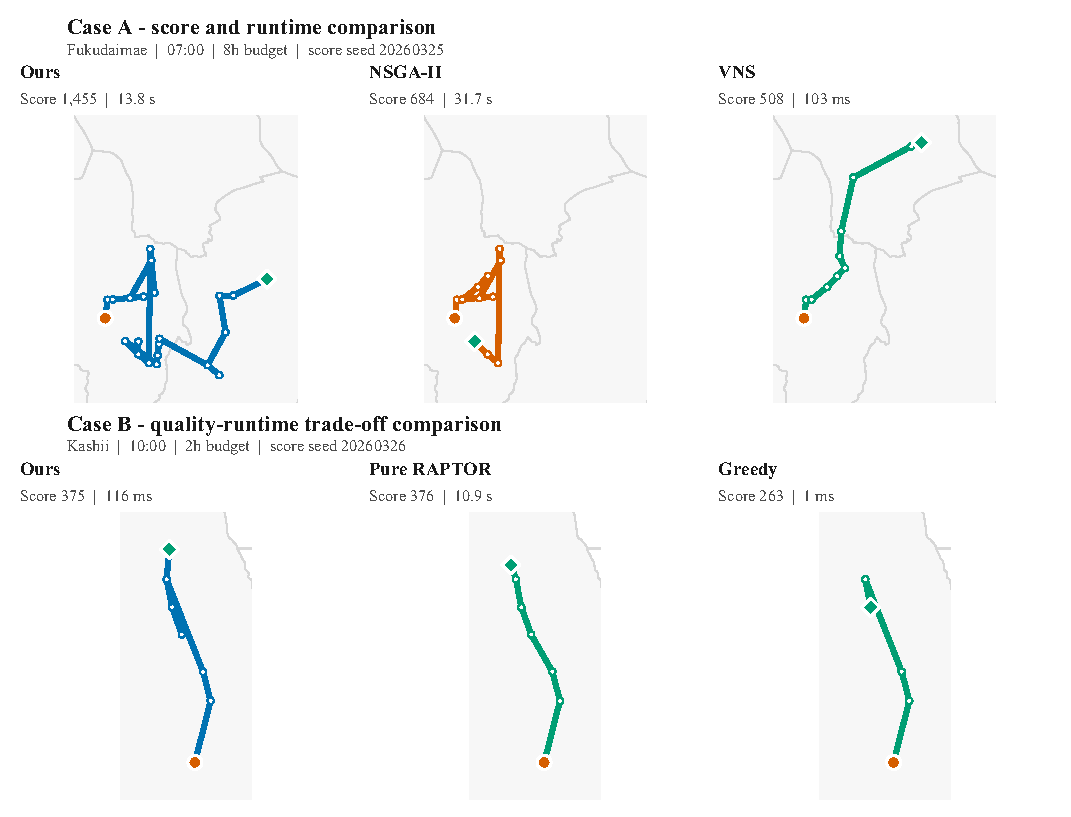
\includegraphics[width=0.96\linewidth]{../figures/exp4/exp4_main_cases.pdf}
\end{center}

\clearpage
\suppheading{Figure S1 (continued)}{Counterexample map}

\begin{center}
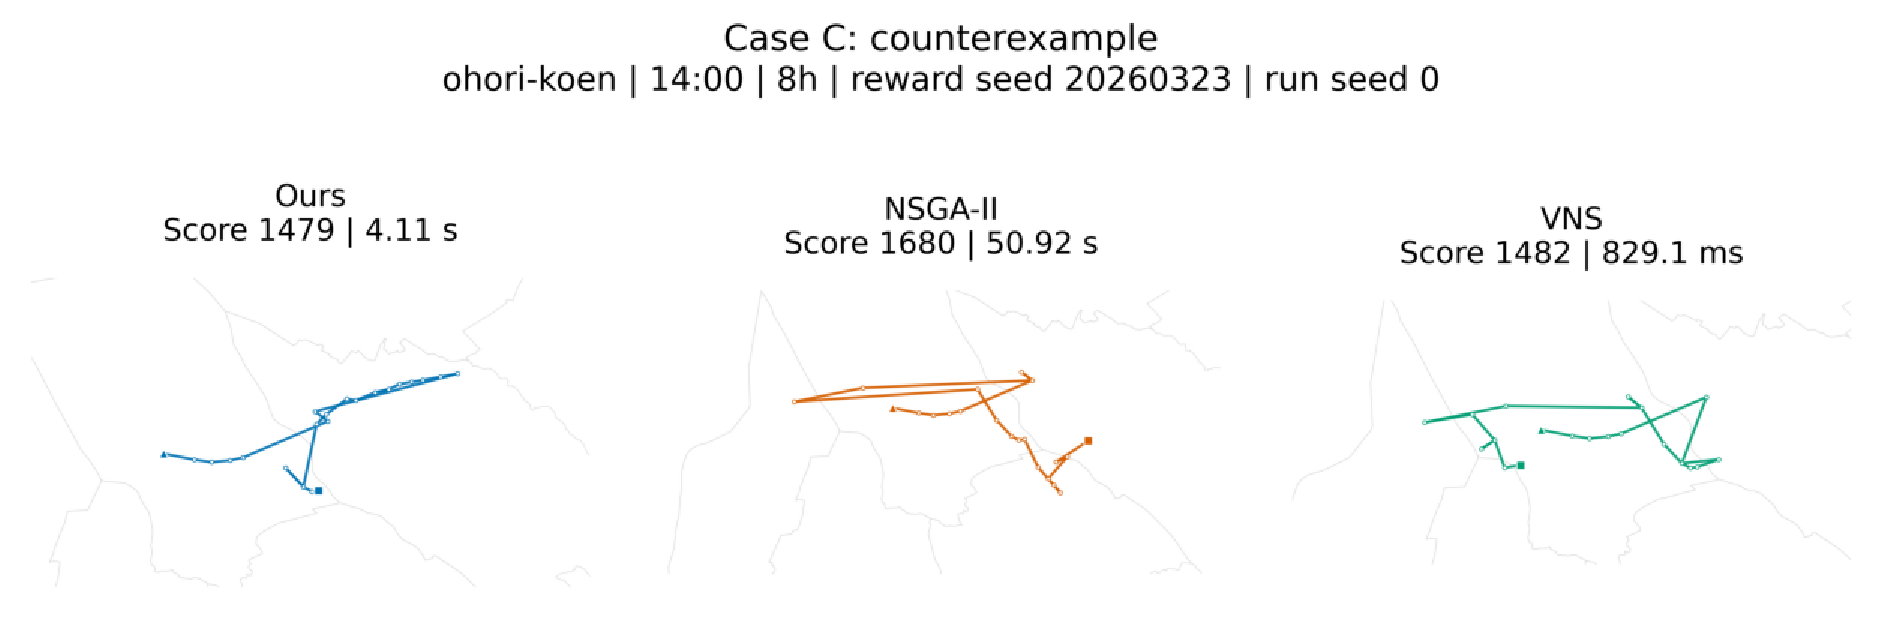
\includegraphics[width=0.96\linewidth]{../figures/exp4/exp4_appendix_cases.pdf}
\end{center}

\sourcefile{paper/figures/exp4/exp4\_main\_cases.pdf}
\sourcefile{paper/figures/exp4/exp4\_appendix\_cases.pdf}
\sourcefile{paper/results/exp4\_route\_visualization/exp4\_cases.json}
\suppheading{Table S7}{Fixed baseline configurations}

\footnotesize
\begin{longtable}{@{}>{\raggedright\arraybackslash}p{22mm}
>{\raggedright\arraybackslash}p{88mm}
>{\raggedright\arraybackslash}p{56mm}@{}}
\toprule
Method & Fixed configuration used in Experiment 1 & Executable specification \\
\midrule
\endfirsthead
\toprule
Method & Fixed configuration used in Experiment 1 & Executable specification \\
\midrule
\endhead
NSGA-II & Population 100; at most 200 generations or 60 s; binary tournament,
nondominated sorting and crowding; timetable-feasible crossover; tail-regrowth
mutation probability 0.22; seeds 0--4. &
\path{paper/experiments/algorithms/nsga2.py}; constants in
\path{paper/experiments/common/config.py}. \\
ILS+2-opt & Timetable-feasible cut-and-tail regrowth; 8--26 local trials per
round; stop after 28 non-improving rounds or 60 s; seeds 0--4. &
\path{paper/experiments/algorithms/ils_2opt.py}. \\
VNS & Four neighborhood strengths; at most four repeated tail perturbations;
stop after 32 stagnant rounds or 60 s; seeds 0--4. &
\path{paper/experiments/algorithms/vns.py}. \\
SA & Initial temperature 1000; cooling 0.995; tail-regrowth neighborhood; stop
below \(10^{-3}\), after 600 stagnant iterations, or after 60 s; seeds 0--4. &
\path{paper/experiments/algorithms/sa.py}. \\
McRAPTOR & Sample 50 destinations per seed, run the simple multicriteria RAPTOR
journey query, retain the resource-feasible route with highest benchmark search
score; seeds 0--4. &
\path{paper/experiments/algorithms/mcraptor.py}. \\
Pure RAPTOR & ReRAPTOR scheduled-edge expansion with candidate trimming, bucket
beam, Dominance, and Negative down-ranking disabled; 60-s guard; deterministic. &
\path{paper/experiments/algorithms/pure_raptor.py}. \\
Greedy (\(L=3\)) & Score up to nine immediate candidates; add the best three
one-step onward candidates with discount 0.3; 60-min immediate and 30-min
onward lookahead; deterministic. &
\path{paper/experiments/algorithms/greedy.py}. \\
ALNS (adapted) & Four destroy--repair operators; 160 iterations or 45 s;
operator-weight update every 12 iterations; \(T_0=6\), cooling 0.985, floor
0.6; seeds 0--4. &
\path{paper/experiments/algorithms/zhou_wang_2025_alns_adapted.py}. \\
DynPref (adapted) & Utilization thresholds 0.35 and 0.70; exploration rates
0.50/0.38/0.22; stop after 24 failed repairs or 45 s; seeds 0--4. &
\path{paper/experiments/algorithms/zhang2025_dynamic_pref_adapted.py}. \\
\bottomrule
\end{longtable}

All methods use the same timetable-feasibility checker, three-minute transfer
buffer, Stop Score map, per-stop effective-time charge, and post-return
validator. Deterministic methods run once per matched task; stochastic methods
are averaged over seeds 0--4.

\sourcefile{paper/results/exp1\_algorithm\_comparison/exp1\_results\_canonical\_final\_10alg\_manuscript\_20260723.json}
\sourcefile{paper/experiments/common/config.py}
\end{document}
